\documentclass{article}
\usepackage{float}
\usepackage{arxiv}
\usepackage{graphicx}
\usepackage[utf8]{inputenc} % allow utf-8 input
\usepackage[T1]{fontenc}    % use 8-bit T1 fonts
\usepackage{hyperref}       % hyperlinks
\usepackage{url}            % simple URL typesetting
\usepackage{booktabs}       % professional-quality tables
\usepackage{amsfonts}       % blackboard math symbols
\usepackage{nicefrac}       % compact symbols for 1/2, etc.
\usepackage{microtype}      % microtypography
\usepackage{lipsum}
\usepackage{subfig}
\usepackage{caption}
\usepackage{subcaption}
\usepackage{csquotes}
\usepackage{listings}

\newcommand{\pasa}{PASA}
\newcommand{\mnras}{Monthly Notices of the Royal Astronomical Society}
\newcommand{\aap}{Astronomy and Astrophysics}
\newcommand{\apjl}{Astrophysics Journal Letters}
\newcommand{\ptrsl}{Philosophical Transactions of Royal Society}

\usepackage[
backend=bibtex,
style=authoryear-icomp,
sorting=ydnt
]{biblatex}
\addbibresource{ref.bib}

\captionsetup[figure]{labelfont=it,textfont={it}}
%\captionsetup[subfigure]{textfont=normalfont,singlelinecheck=off,justification=center}

\title{TIMING AND ANALYSIS of MILLISECOND PULSARS\\ \textit{B.Tech. Project Fall 2021}}



\author{\Large
  Divyansh Kharbanda \\
  EP19BTECH11002\\
  Engineering Physics\\
  Indian Institute of Technology, Hyderabad \\\\
  \textit{Supervisor} : Dr. Shantanu Desai
}
\begin{document}

\begin{center}

\includegraphics[width=0.75\textwidth]{Images/horzlogolong.png}
\end{center}
\maketitle 

\newpage
\tableofcontents
\newpage
\begin{abstract}
 The pulsar timing array experiment (PTA) employs an ensemble of millisecond pulsar clocks to detect gravitational waves. PTAs are expected to open the nano-Hertz window of the gravitational wave spectrum. Although the millisecond pulsars are known to be very stable rotators, on rare occasions there could be irregularities such as glitches, extreme scattering events, profile changes, etc seen in these pulsars. Monitoring such events and their recovery is crucial for modelling the noise processes in pulsar data sets used in PTAs. (\cite{taylor2021nanohertz})

This report summarizes the work I have done, while contributing to the Indian Pulsar Timing Array (InPTA) group, under the guidance of Prof. Shantanu Desai. InPTA is an Indo-Japanese consortia consisting of members from NCRA-TIFR, TIFR, IMSC, IIT Hyderabad, IIT Roorkee, BITS Hyderabad, Kumamoto University and  led by Prof. B.C. Joshi (NCRA)  and has been observing pulsars since 2014. The objective of InPTA is to detect, analyse and study nanoHertz Gravitational Waves. While having monitored a few observations remotely, the bulk of my contribution lies in the analysis of the observed pulsar data. 
\end{abstract}
\newpage

\section{INTRODUCTION}
\subsection{PULSARS}
Pulsars are a special class of neutron star, which themselves correspond to the collapsed $M_o$ cores of massive stars that have undergone supernovae, leaving only small (10-15 km) carcasses with masses of $1-2 M_{\odot}$ that are supported against total collapse by neutron degeneracy pressure. They emit beams of radiation from their magnetic poles, which is observed mainly in the radio, X-ray and gamma spectrum.
\\
Pulsars have shed light on strong-field gravity,
the equation of state of nuclear matter, evolutionary scenarios for massive binary systems, the
structure of the ionized interstellar medium, the existence of exoplanets, and much more.

The “lighthouse model” provides our basic framework for understanding and modeling pulsars as rapidly rotating, highly magnetized neutron stars resulting from stellar collapse. Due to conservation of angular momentum and magnetic flux, these pulsars are far more rapidly spinning and magnetized than their progenitor stars.
\begin{figure}[h!]
\begin{center}
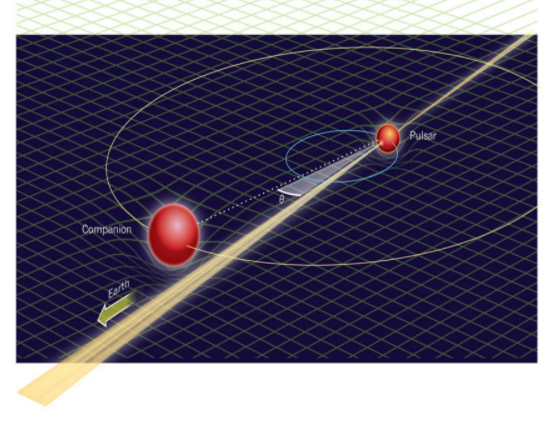
\includegraphics[height=4cm,width=7cm]{Images/Pulsar1.png}
\caption{Diagrammatic Representation Shapiro Delay (Source : Manjari Bagchi, InPTA Student Week 2021)}
\end{center}
\end{figure}
Their magnetic field (whose axis may not necessarily align with its rotational axis) is such that the star acts as a rotating magnetic dipole, generating a local electric field along which charged particles within the
co-rotating magnetospheric plasma are accelerated. It is expected that these particles excite beams of radio emission high in the pulsar atmosphere that we observe whenever the rotating beam intersects our line-of-sight. The pulse period is then a measure of the rotation period of the pulsar itself.

\begin{figure}[h!]
\begin{center}
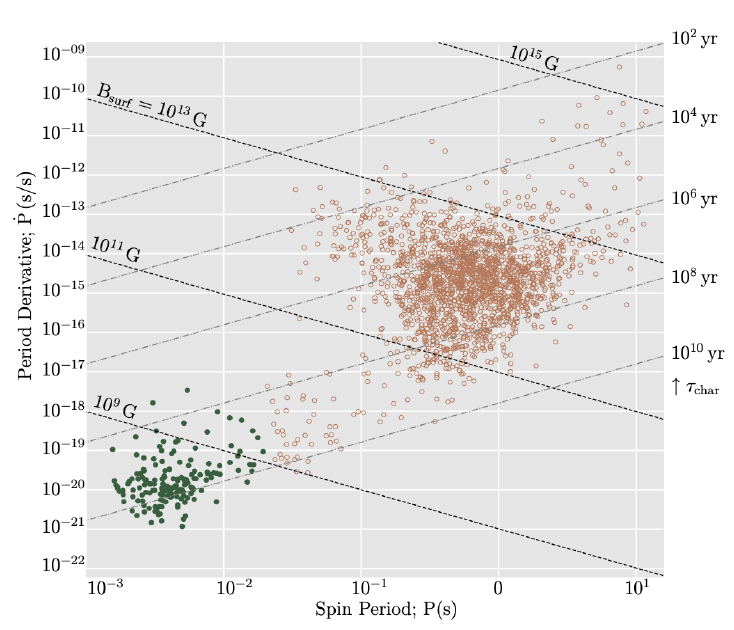
\includegraphics[height=6cm,width=7cm]{Images/V2_3.png}
\end{center}
\caption{
$P - \dot{P}$ diagram of known pulsars. Millisecond pulsars are filled green circles, while canonical pulsars are open circles. The dashed black lines show estimated surface magnetic fields strengths ($B_{surf}$), while the dot-dashed grey lines show the lines of characteristic age. Data were taken from the ATNF pulsar catalogue [11] version 1.56} (\cite{taylor2021nanohertz})
\end{figure}

\newpage
\subsection{PULSAR TIMING}
We observe the pulses of radio emission separated by the observational period of the pulsar. However, the shape of each pulse from one rotation to the next varies randomly, possibly associated with stochasticity in the emission region through which our line of sight traverses. But the pulse shape averaged over the rotations is remarkably stable and reproducible on timescale from minutes to decades. It is this stability at a given radio frequency that permits precision timing; the pulse shape is unique to each pulsar and can be relied upon to mark the passage of rotations when receiving a train of radio pulses. (\cite{taylor2021nanohertz})\\

\begin{figure}[htbp] % H here makes the images come at the correct position
\centering
\begin{minipage}{.5\textwidth}
  \centering
  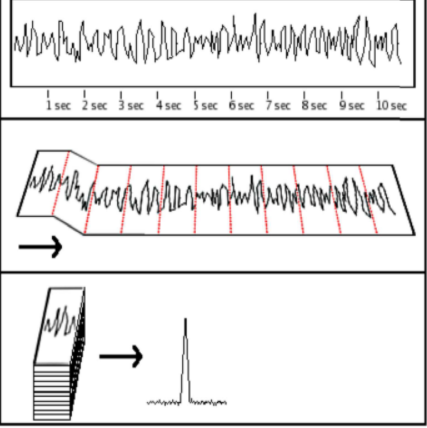
\includegraphics[width=0.7\linewidth]{Images/Pulsar2.png}
  \captionof{figure}{Ryan Lynch: Pulsar searching tutorial for PSC}
\end{minipage}%
\begin{minipage}{.5\textwidth}
  \centering
  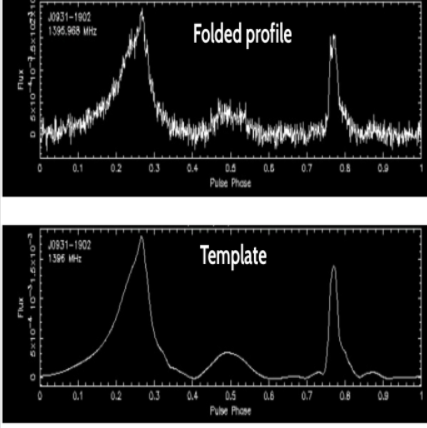
\includegraphics[width=0.7\linewidth]{Images/Pulsar3.png}
  \captionof{figure}{James McKee: Pulsar timing tutorial, IPTA 2018 student week}
\end{minipage}
\end{figure}

Pulsar Timing involves tracking the pulsar rotation by measuring pulse arrival times (TOAs).  Through these time of arrivals, we calculate  the time of emissions at the pulsar. The complications involved in this calculation include:

\begin{enumerate}
  \item Pulsars slow down, hence the emission times are not constant. We fit our models to obtain the true fit for time of emissions.
  \item The space between the pulsar and the Earth is not vacuum, but is the interstellar medium (ISM). This  causes the pulse to travel at sub-light-speed, dependent on the frequency of the spectrum. The pulse is composed of a band of frequencies, each of which experiences this phenomena. To obtain the correct results,   the whole band is divided into N channels, data recorded at these channels, the added. Signals at different channels arrive at different times - addition will not give a good signal. We need to correct for this dispersive delay to get a good pulse.
  \item Romer delay due to the motion of the Earth around the sun. 
  \item Effects arising out of special and general relativity :
    \begin{enumerate}
        \item Curvature of space time due to masses of other planets in our solar system, any companion to the pulsar and the pulsar itself. 
        \item Motion of the pulsar relative to our planet. 
    \end{enumerate}
\end{enumerate}

The Romer, Einstein, and Shapiro delays all contribute to the difficulties in the analysis. To ensure uniform and complete analysis of the data, a data processing pipeline was developed by the InPTA for use.
%SD: please add references for Romer, Einstein and Shapiro delay
\newpage

\subsection{uGMRT : Upgraded Giant Metrewave Radio Telescope}
The pulsars are observed by the Upgraded Giant Metrewave Radio Telescope (uGMRT), located near Pune at Khodad and is operated by the National Centre for Radio Astrophysics, TIFR.\\
The antennas form an interferometric array, which is composed of a total of 30 antennas: 14 in the central square and 16 distributed in a Y-shaped arm.
Each antenna is a parabolic reflector having a diameter of 45 metres.
The uGMRT provides a frequency coverage from 30 MHz to 1500 MHz. Simultaneous multi-band observations across four bands with high sensitivity with an instantaneous bandwidth of 400 MHz. (\cite{10.2307/26293915})
\begin{figure}[htbp]
\begin{center}
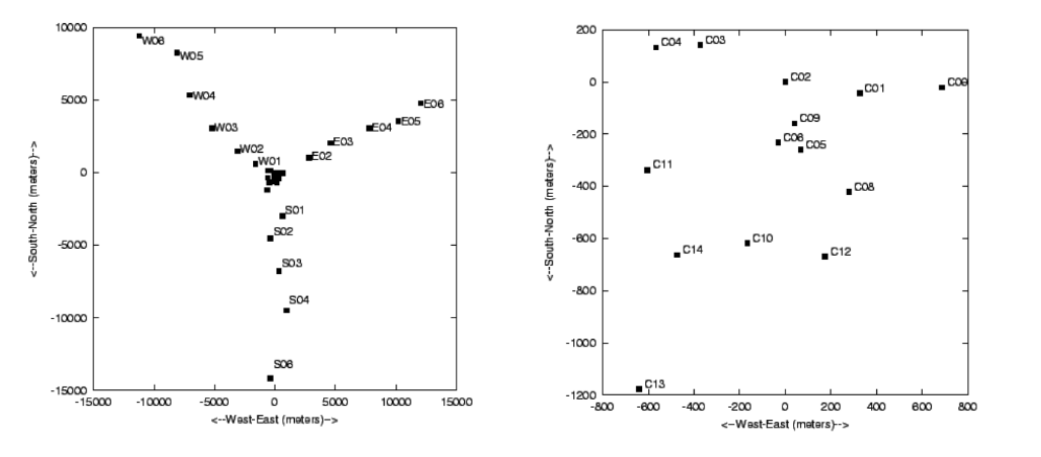
\includegraphics[width=0.75\textwidth]{Images/V2_1.png}
\caption{Layout of Antennas at the uGMRT (Credit : NCRA-TIFR)}
\end{center}
\end{figure}
\\
The uGMRT has four bands which allow for simultaneous wideband observations in multiple bands:
\begin{enumerate}
    \item BAND 5: 1000 to 1500 MHz
    \item BAND 4: 550 to 900 MHz
    \item BAND 3: 250 to 500 MHz
    \item BAND 2: 120 - 250 MHz
\end{enumerate}

InPTA has observed it’s pulsars in bands 3, 4 and 5. 
Recent cycles have had observations in bands 3 and 5.
The 30 antennas of GMRT are split into 2 (or 3) sub-arrays, where each sub-array observes sources in a different band. Observations occur with a bandwidth of 100 or 200 MHz. 
\begin{figure}[htbp]
\begin{center}
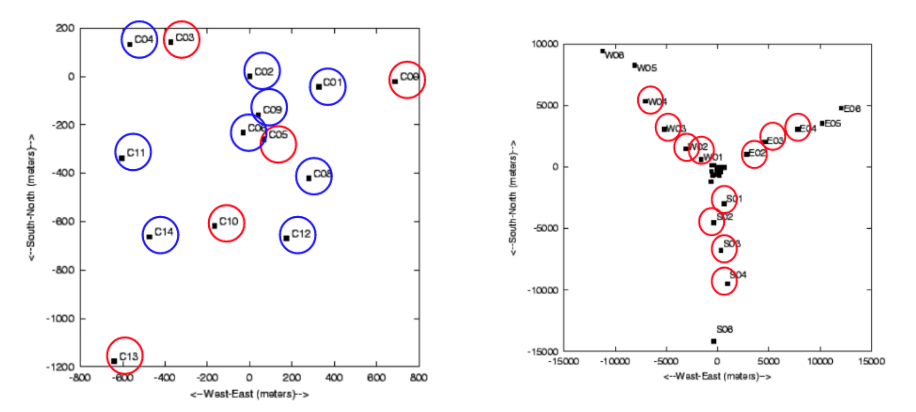
\includegraphics[width=0.75\textwidth]{Images/V2_2.png}
\caption{The above  image shows an setup with blue antennas observing in BAND3, with red antennas observing in BAND 5. (Credit : NCRA-TIFR)}
\end{center}
\end{figure}
\newpage
\subsection{PINTA}
PINTA, which stands for the "Pipeline for the Indian Pulsar Timing Array" is the software developed for the InPTA experiment to address these concerns as well as to improve the efficiency, reliability, and user friendliness of the data reduction process and to ensure faster turnaround time from observations to PTA analysis.  This allows for the homogeneity in data reduction practices to avoid non-uniformity in the data products used for PTA analysis, which can introduce systematic errors. (\cite{Susobhanan+2021})
\begin{figure}[htbp]
\begin{center}
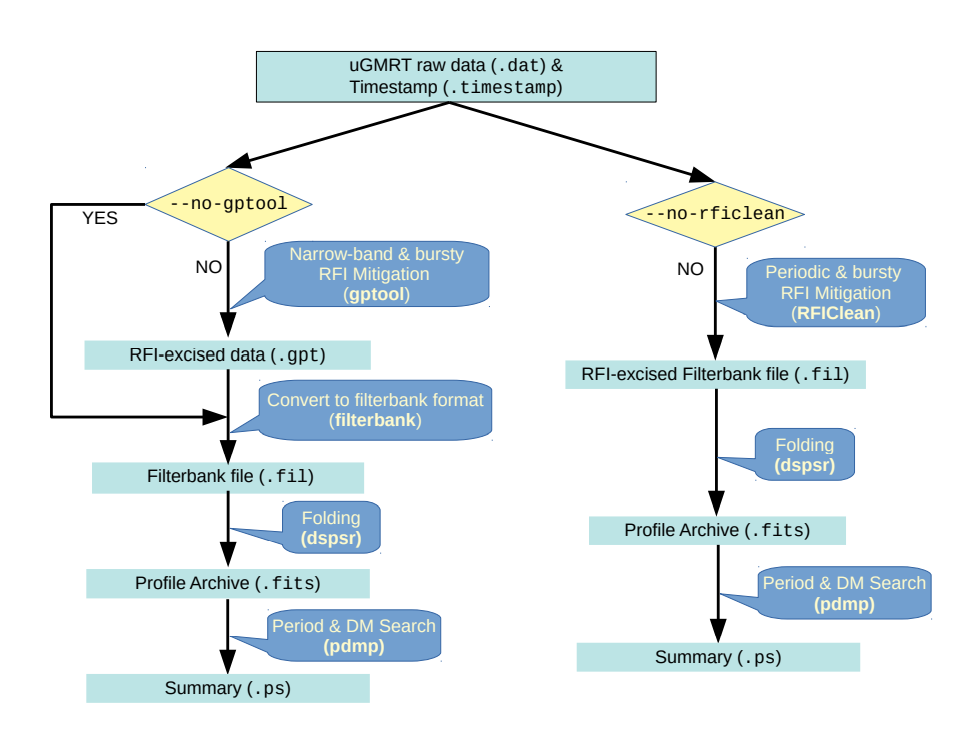
\includegraphics[height=7cm,width=8cm]{Images/Pulsar4.png}
\caption{The workflow of pinta. The pinta pipeline uses uses two separate packages for the RFI mitigation, namely gptool and RFIClean. A typical data reduction workflow can optionally engage these RFI mitigation choices. Note that the profile archives generated by pinta are in the Timer format although their extension is ‘.fits’. (\cite{Hotan+2004})}
\end{center}
\end{figure}
\\\textbf{gptool} : It is both an RFI mitigation and a data reduction tool for the beamformer data from GMRT. It mitigates both narrow-band spectral line RFI and broadband bursty time-domain RFI.
\\\textbf{RFIClean} : It  excises periodic RFI in the Fourier domain, and then mitigates narrow-band spectral line RFI and broadband bursty time-domain RFI using robust statistics of conventional RFI mitigation techniques.
\begin{figure}[htbp]
\begin{center}
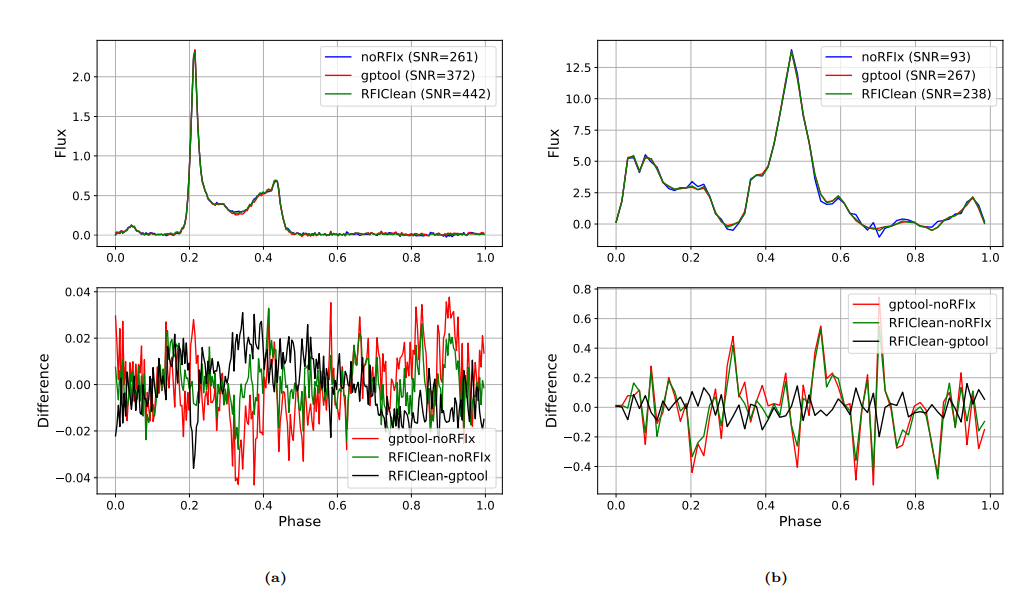
\includegraphics[height=6cm,width=14cm]{Images/V2_6.png} 
\caption{Comparison of frequency collapsed profiles obtained using gptool, RFIClean, and without any RFI mitigation (noRFIx).Both epochs show significant improvement in SNR while using RFI mitigation. (a) PSR J2145-0750 observed on 16 June 2020 in Band 5 (1260-1460 MHz) with 40.96 µs sampling time and no coherent dedispersion. The total integration time is 55 min. (b) PSR J2124-3358 observed on 25 August 2018 in Band 3 (400-500 MHz) with 81.92 µs sampling time with coherent dedispersion. The total integration time is 24 min (\cite{Susobhanan+2021})}
\end{center}
\end{figure}

\clearpage
\newpage
\subsection{PROCESSING INDIVIDUAL EPOCHS}
The processing pipeline takes in  .raw/.dat files and timestamps, as obtained from an observation as its input. It also takes in a pipeline.in file containing the metadata parameters with which to process the raw data files. The resulting output is in the form of archive files, a pulsar data format widely used among other PTAs. (\cite{Susobhanan+2021})
\\
The pipeline is made up of multiple softwares, which perform the functions of de-dispersion, folding, Single Pulse Analysis,  RFI cleaning, Template making, ToA generation, Flux calibration and Pulsar Calibration; to obtain the accurate results.

The primary processing of pulsar data results in an output that looks like the following. It can easily be observed that a pulsar was detected in the first observation, while it was not in the second one (note the pulse shape in the bottom plot).\\

\begin{figure}[htbp] % H here makes the images come at the correct position
\centering
\begin{minipage}{.5\textwidth}
  \centering
  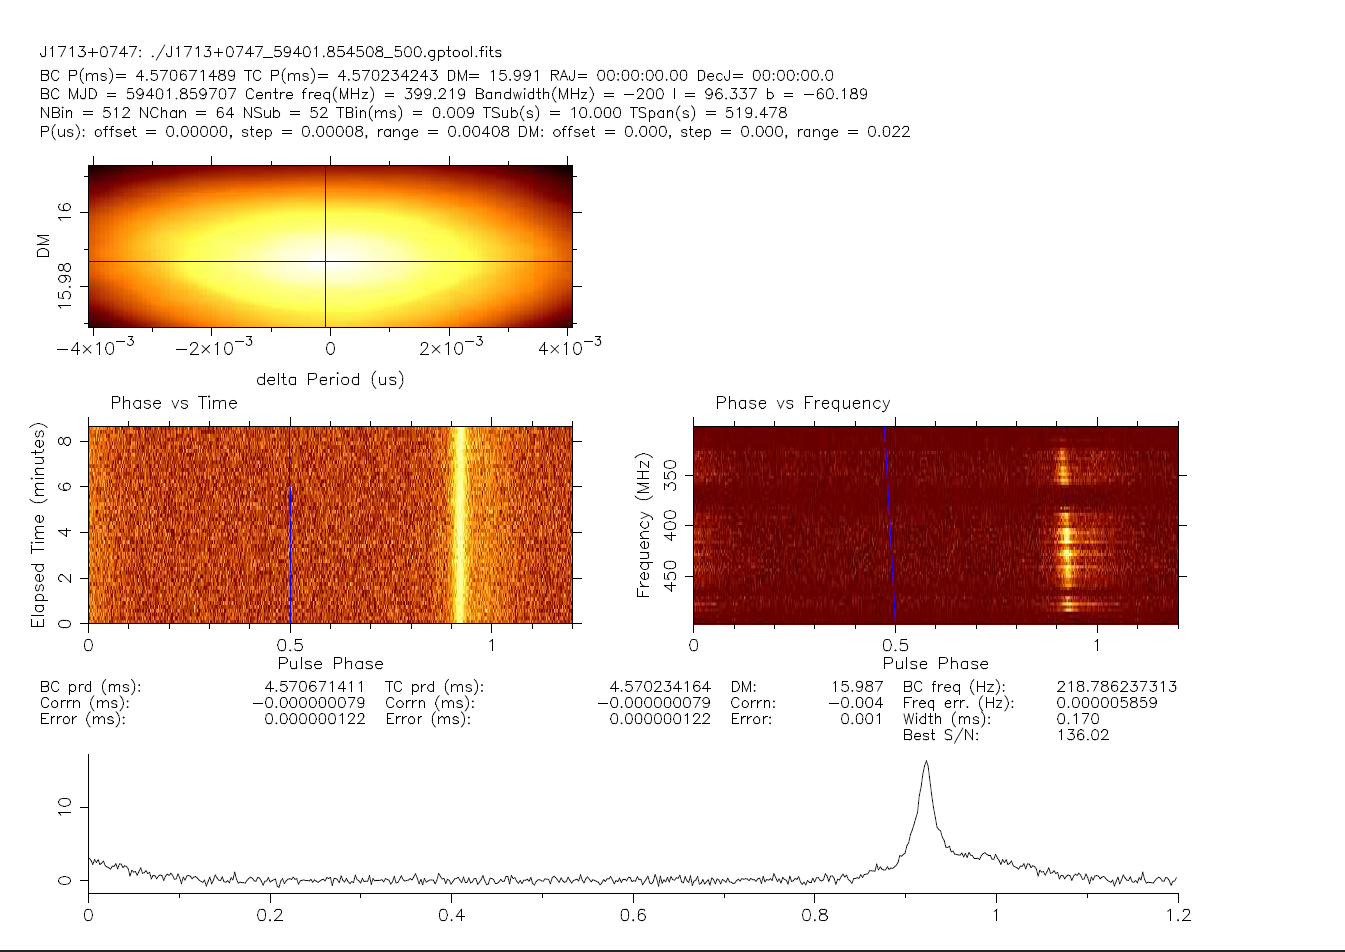
\includegraphics[width=0.9\linewidth]{Images/Pulsar5.png}
  \captionof{figure}{Output from the gptool processing of an observation data on Jul 07 (monitored on by me)}
\end{minipage}%
\begin{minipage}{.5\textwidth}
  \centering
  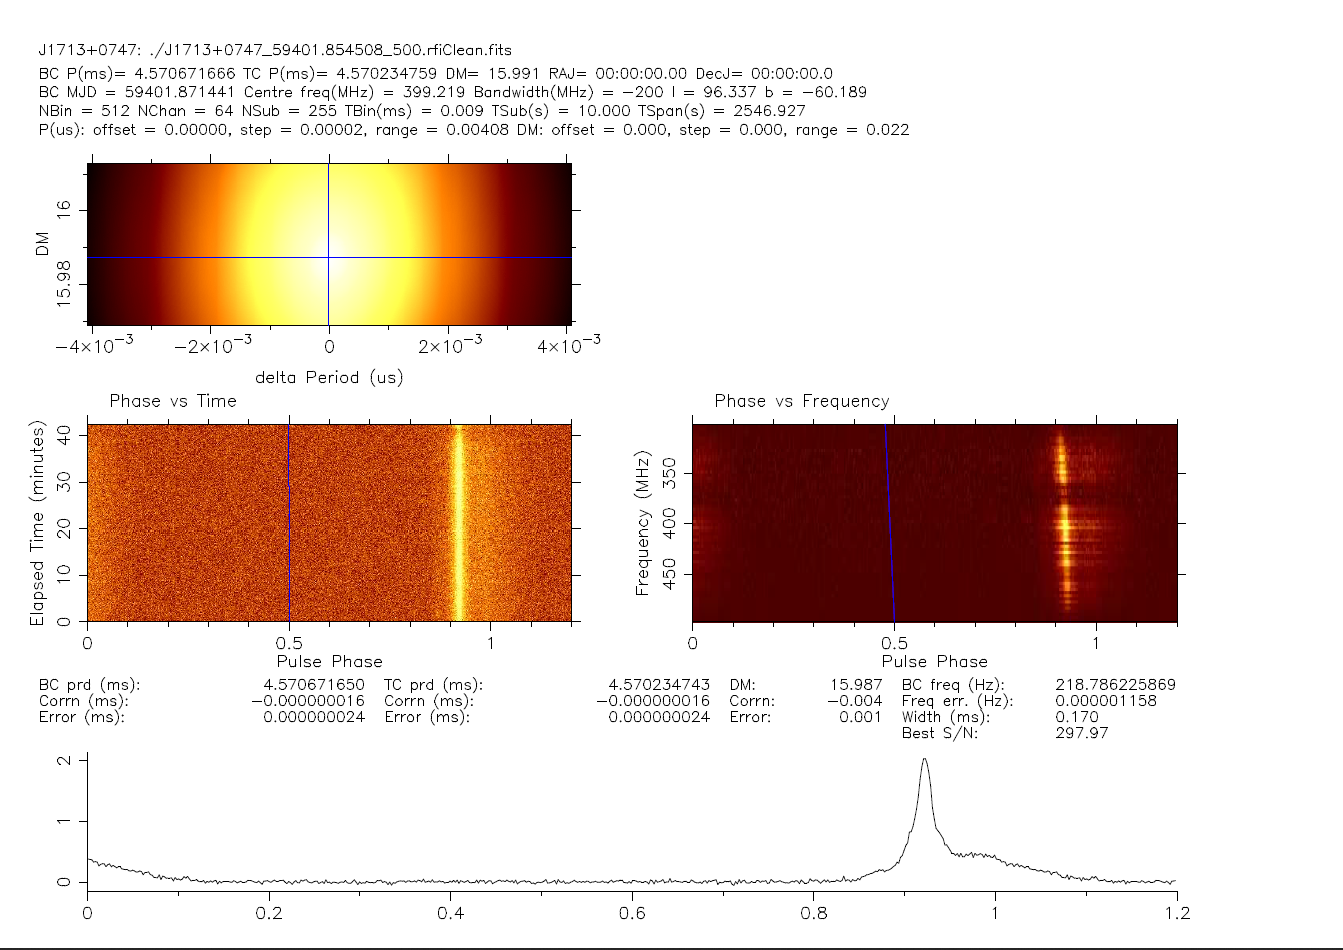
\includegraphics[width=0.9\linewidth]{Images/Pulsar6.png}
  \captionof{figure}{Output from rfiClean processing of an observation data on Jul 07 (monitored on by me)}
\end{minipage}
\end{figure}
% Divider line here
\begin{figure}[htbp] % H here makes the images come at the correct position
\centering
\begin{minipage}{.5\textwidth}
  \centering
  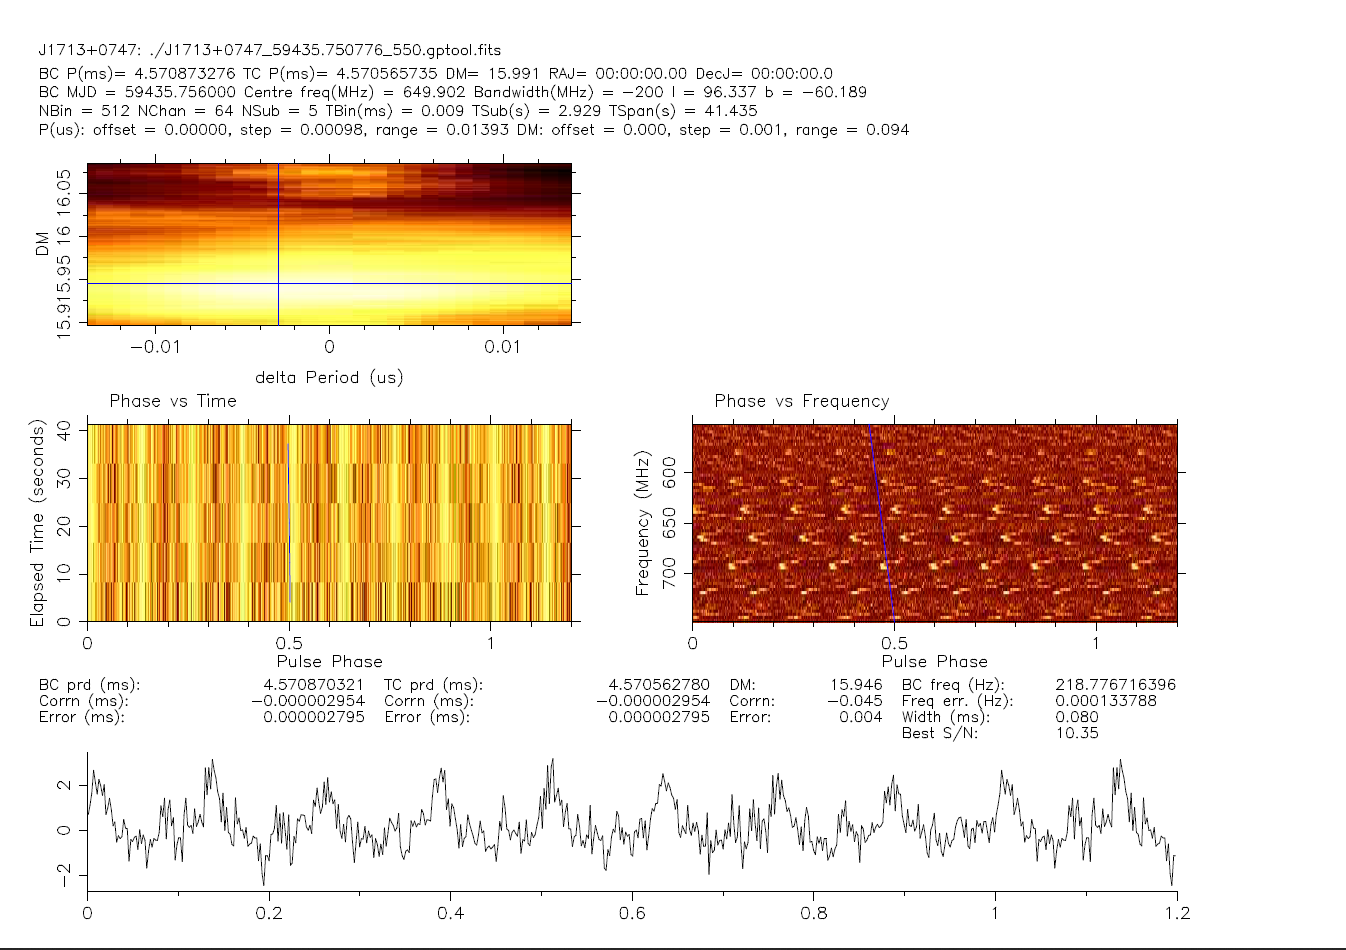
\includegraphics[width=0.9\linewidth]{Images/Pulsar7.png}
  \captionof{figure}{Output from the gptool processing of an observation data on Aug 09 2021 (monitored on by me) }
\end{minipage}%
\begin{minipage}{.5\textwidth}
  \centering
  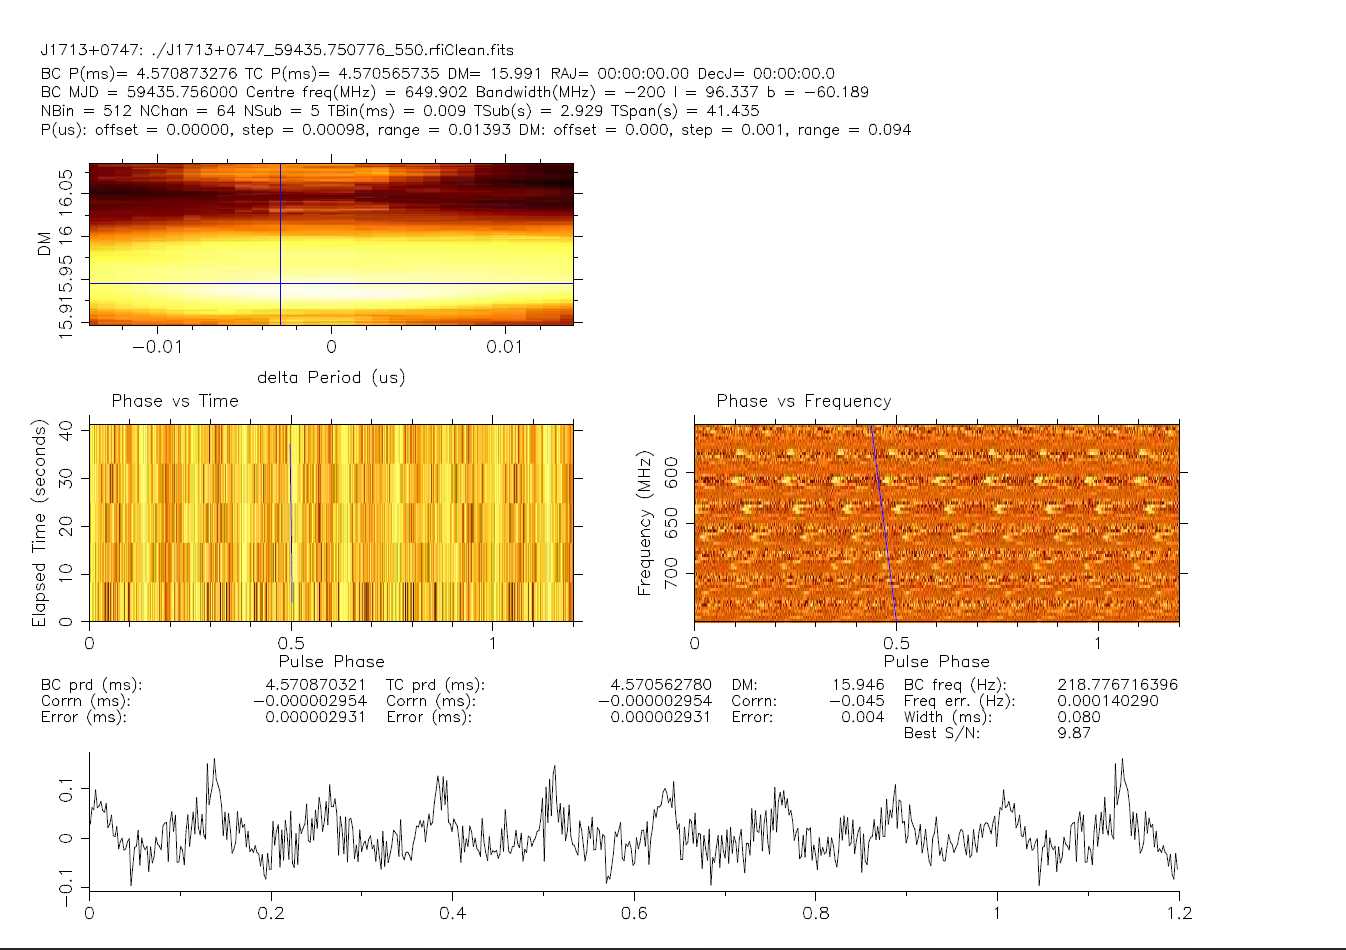
\includegraphics[width=0.9\linewidth]{Images/Pulsar8.png}
  \captionof{figure}{Output from the rfiClean processing of an observation data on Aug 09 2021 (monitored on by me) }
\end{minipage}
\end{figure}
The process of observation itself requires careful consideration of the rise and set time of pulsars, optimal choice of phasing sources to calibrate the antennas, awareness of sources of radio frequency interference like satellites, which can pass nearby and affect the observations itself. Such careful measures are necessary in the art of pulsar analysis, and are the reason why most of the observations do not yield unusable results. \\
\clearpage
\newpage

\subsection{OVERVIEW OF PROCESSING}
The figure below summarizes the entire procedure followed from observation to folding, pre-processing, processing to analysis. 
\begin{figure}[htp]
    \centering
    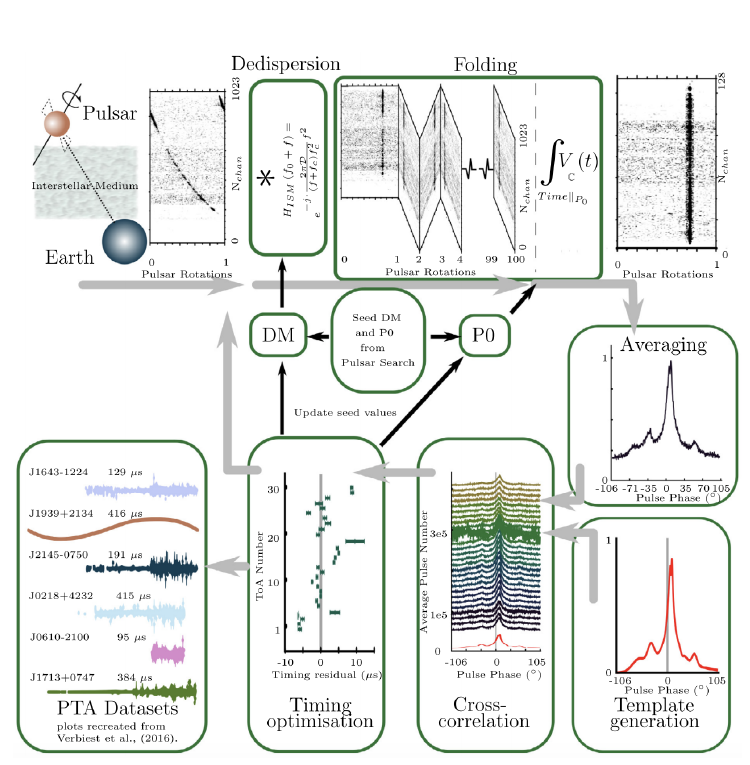
\includegraphics[height=12cm,width=12cm]{Images/V2_4.png}
    \caption{A representation of the main stages involved in the precision timing of pulsars. (\cite{taylor2021nanohertz})}
\end{figure}

\subsection{CONTRIBUTIONS TO InPTA}
My work on  INPTA  is summarized below:
\begin{enumerate}
\item My contributions over the recent months have been the processing of Pulsar Data using the Pinta pipeline, which was used under the team effort to collect evidence for the profile changes in pulsar J1713+0747. I was also involved in a couple of pulsar observations under the same effort. This work has been published in MNRAS~\cite{10.1093/mnrasl/slab098}.

\item When it was recognised that there might be an issue with the configuration processes of the Pinta pipeline itself, I was part of the subgroup that was set-up to validate the effects of various configurations of the data processing software. 

\item During the same time, it was noticed that there was a discrepancy in the DMs of the processed data. I was given the task to find out the exact difference and report the same (which was then incorporated into the observation process itself). The results of this study have been used by the GMRT team to issue a technical note regarding the frequency shift.

\item I am continuing  to participate in observations, data reduction and backup during ongoing Cycle 41 observations. 
\end{enumerate}
\clearpage
\newpage
%%%%%%%%%%%%
\section{EVIDENCE FOR PROFILE CHANGES IN PSR J1713+0747 USING THE UGMRT}
\label{sec:headings}
 \subsection{INTRODUCTION}
PSR J1713+0747 is a 4.6 ms pulsar with a low-mass white dwarf companion (\cite{FosterWC+1993}), and has the second lowest measured timing noise behaviour in the PTA ensemble (\cite{pdd+19}), making one of the most precisely timed pulsars in the international pulsar timing array experiment. This pulsar showed an abrupt profile shape change between 2021 April 16, (MJD 59320) and 2021 April 17 (MJD 59321). My contribution in the group effort to report the results involved processing multiple batches of pulsar data. 

\begin{figure}[htbp]
\centering
\begin{minipage}{.5\textwidth}
  \centering
  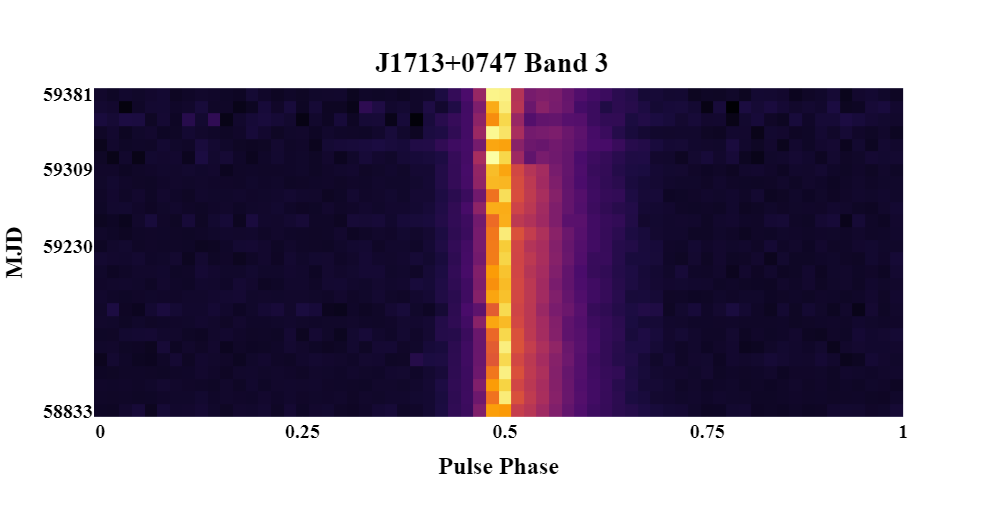
\includegraphics[width=\linewidth]{Images/Pulsar10.png}
  \captionof{figure}{Band 3 Phase Change Plot}
\end{minipage}%
\begin{minipage}{.5\textwidth}
  \centering
  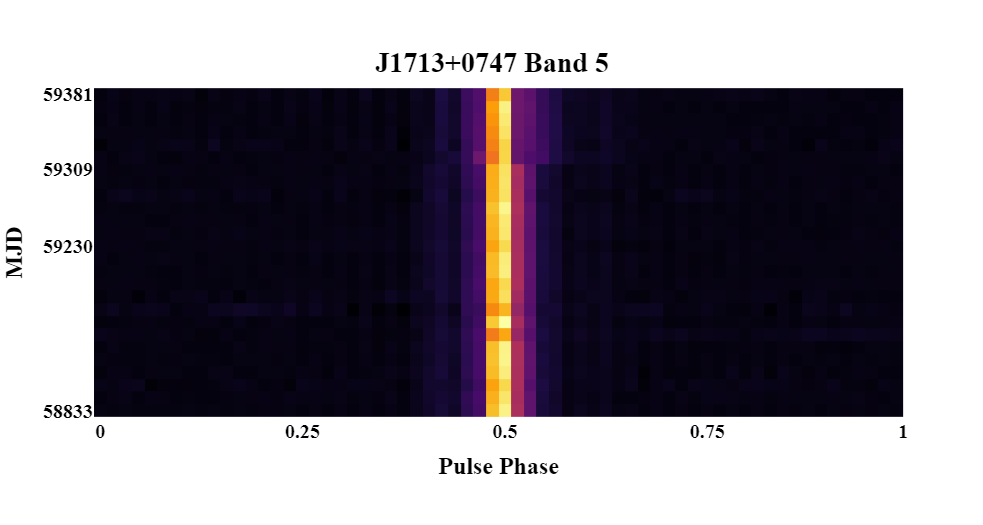
\includegraphics[width=\linewidth]{Images/Pulsar11.png}
  \captionof{figure}{Band 5 Phase Change Plot}
\end{minipage}
\end{figure}

\subsection{OBSERVATIONS}
PSR J1713+0747 was observed with the uGMRT (\cite{Gupta+2017}) as part of the InPTA (\cite{JoshiAB+18}) observing program before and after the profile change event reported here, as well as via a Director’s Discretionary Time (DDT) project after the event. The InPTA observations were carried out using two sub-arrays of 10 and 15 antennae at 300–500 MHz (Band 3) and 1260–1460 MHz (Band 5), respectively.\\

All observations used 200 MHz bandwidth. This bandwidth was split into 256 and 128 sub-bands (before and after MJD 59348, respectively) for Band 3 and 1024 sub-bands for Band 5 observations, respectively.\\

The raw time-series were further reduced to Timer format (\cite{vanStratenBailes2011}) using the pinta pipeline (\cite{Susobhanan+2021}). Further analysis was carried out using the widely-used pulsar software {\tt PSRCHIVE} (\cite{Hotan+2004}). The time-series were folded using pulsar ephemeris derived from the IPTA Data Release 2 (\cite{Perera+2019}). Out of the two radio-frequency mitigation methods available in pinta, we exclusively used RFIClean (\cite{Maan+2020})in this work.

\clearpage
\newpage
\subsection{THE PROFILE CHANGE}
We used 20 observing epochs before the event with a cadence of around 14 days, and 6 epochs after the event with cadence ranging from 3–10 days. After de-dispersion and collapsing all the sub-integrations and sub-bands, the folded profiles were normalized with the area under the profile and then stacked together to produce a single multi-epoch file for each of Band 3 and 5. These stacked profiles are shown as color-map plots. 

\begin{center}
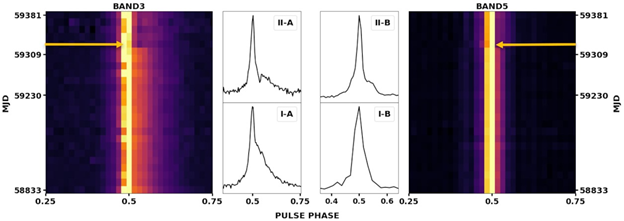
\includegraphics[height=5cm,width=12cm]{Images/Pulsar12.png}\\
\end{center}
A distinct change is seen in both Band 3 and Band 5 before and after MJD 59321, reported to be the epoch of the event (\cite{Meyers+2021}). The reduced data were collapsed in frequency and time for typical profiles before and after the event for both the bands and these are shown above. 

The degree of change in the profile was quantified through the following process. First, a high signal-to-noise ratio (S/N) template profile was formed by averaging all the profiles before the event. Then, the profiles at individual epochs, both before and after the event, were scaled and shifted to align with this template using a frequency-domain cross-correlation method (\cite{Taylor1992}). The scaled and shifted profiles were then subtracted from the template to form profile differences, and were examined for significant deviations. The results of this process can be viewed in the following plot. 
\begin{center}
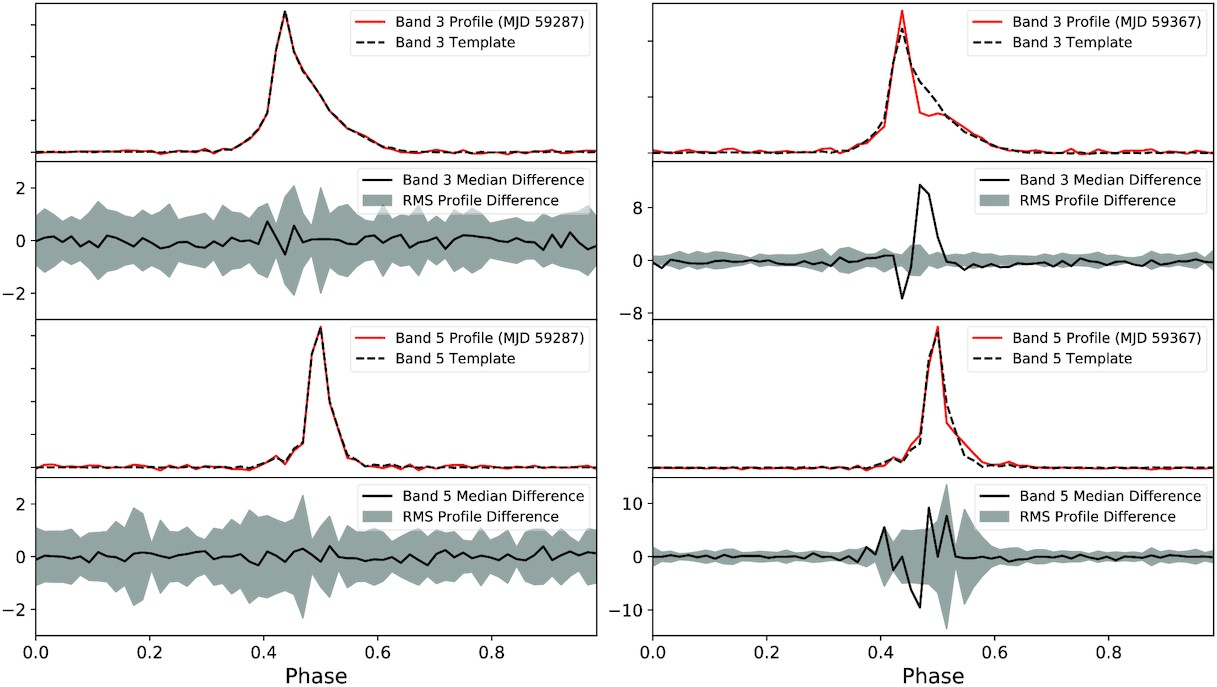
\includegraphics[height=6cm,width=14cm]{Images/V2_5.png}\\
\end{center}
\newpage
\subsection{RESULTS}
The profile change is seen in both Band 3 and Band 5 data after MJD 59321 with a peak deviation of 12 and 8 times off-pulse RMS, and an enhanced variability in Band 5 profiles after the event. This variability appears to be linked with a jump that is followed by an exponential recovery seen in the timing residuals with a magnitude of ~48 $\mu s$ and a recovery time-scale of ~159 days. \\\\
We infer that the event is unlikely to be due to a change in the ISM alone as 
\begin{enumerate}
    \item the event appears to be more pronounced in Band 5 than in Band 3 with a chromatic index of ~-1.34
    \item  a profile change is seen in both high and low frequency bands
\end{enumerate} 
Profile mode changes are believed to arise from a re-organization of pulsar beams, probably due to global changes in the pulsar magnetosphere (\cite{Timokhin2010}), and can exhibit quasi-periodicity (\cite{Lyne+2010}) accompanied by changes in the spin-down rate. This leads to higher timing noise (\cite{arun2017}) in the pulsar, which has the potential to degrade the precision achievable for PTA experiments relying on the high stability of MSPs.\\\\
\newpage
\section{PINTA VERSION 6 VALIDATION}
\subsection{INTRODUCTION}
The Data processing pipeline, pinta, receives regular updates from its maintainers. The latest version of the same is version 6, with which a majority of the pulsar data for the year was processed. This processing pipeline runs across multiple production grade servers to help provide maximum work efficiency. However, on upgrading it from version 5 to version 6, a discrepancy was created due to different configuration files being sourced on different servers. This could possibly have affected the processed data.\\
To check if the above mentioned scenario had really created an issue, a plan was formulated to process data from pulsars with high SNR, using configuration files with different parameters (in local server directories), to check the impact of having different/ no configuration file on the processed data.\\
This task was treated with the highest priority for the following reason. In the event that this minuscule change actually affected the processed data, the processed data from their entire batch would have become unfit for use. The raw data for an observation is deleted after its processing to make space for new data, hence multiple observations would have been lost due to this issue.  
\subsection{ACTION TAKEN}
The work was divided to completely reprocess specific epochs of two pulsars J1713+0747 and J1939+2134, as they both had high SNRs. The configuration files were to be identical, with a change in the two parameters : 
\begin{enumerate}
    \item Barycentric Correction (Value could be 0 or 1). 
    \item Rounding Correction (Value could be 0 or 1). 
\end{enumerate}
A subset of the configuration file with the relevant parameters can be seen below :
\begin{lstlisting}
###########################################################################
#
# Append::must_match - Ensure that Archive parameters match [boolean]
#
# If true, then TimeAppend and FrequencyAppend (used by psradd) will fail
# if certain observational parameters do not match (see ArchiveMatch)
#
# Append::must_match = 1
ArrivalTime::default_format = Tempo2
###########################################################################
#
# Dispersion::barycentric_correction - Dedisperse using barycentric freqs [boolean]
#
# If true, interchannel dispersion delays are calculated and corrected
# using barycentric radio frequency values.  The historical psrchive
# behavior was to use topocentric frequencies.
#
Dispersion::barycentric_correction = 1
###########################################################################
#
# WeightedFrequency::round_to_kHz - Round mean frequency to nearest kHz [boolean]
#
# If true, then WeightedFrequency (used by tscrunch and fscrunch)
# will round the weighted mean frequency to the nearest value in kHz
#
WeightedFrequency::round_to_kHz = 0
\end{lstlisting}
One person was to process without the configuration file. This created 5 possible ways of processing a pulsar. I was to process the J1939+2134 pulsar with Bar 1 and Round 0 configuration. The process involved running {\tt pdmp} and pat on V5 and V6 Pinta processed J1909 Pulsar, and {\tt pdmp}, pat and profile comparison on V6 Pinta processed J939 to find any discrepancies. The results obtained were summarized in the following plots.
\begin{figure}[htbp]
    \centering
    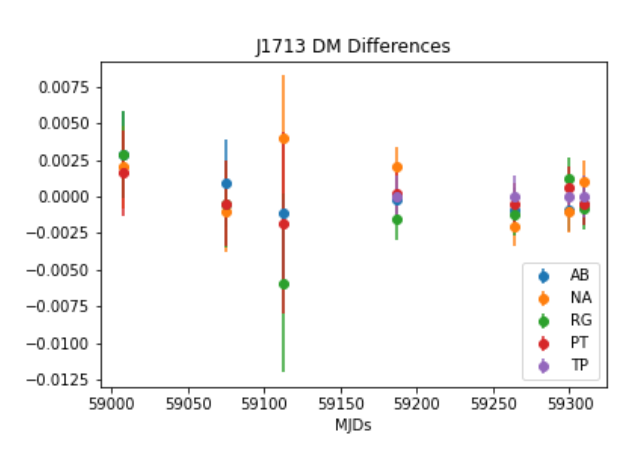
\includegraphics[height=7cm,width=9cm]{Images/V2_9.png}
    \caption{Final Result of DM Differences for Different Configuration files. The legend denotes a separate configuration file for each team member's initials. }
\begin{center}
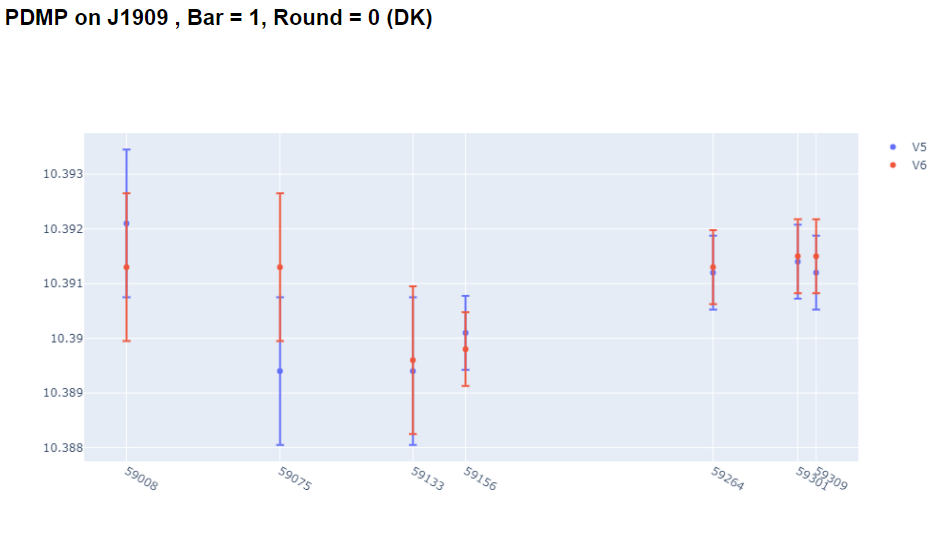
\includegraphics[height=8cm,width=12cm]{Images/Pulsar13.png}
\caption{Result of using the {\tt pdmp} Analysis on J1909 Pulsar, with configuration as Bar = 1, Round = 0, done by me}
\end{center}

\centering
\begin{minipage}{.48\textwidth}
  \centering
  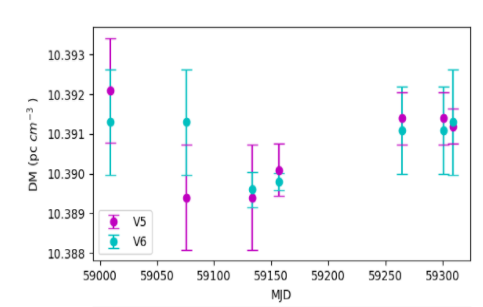
\includegraphics[width=\linewidth]{Images/V2_7.png}
  \captionof{figure}{Result of using the {\tt pdmp} Analysis on J1909 Pulsar, without any configuration}
\end{minipage}%
\begin{minipage}{.52\textwidth}
  \centering
  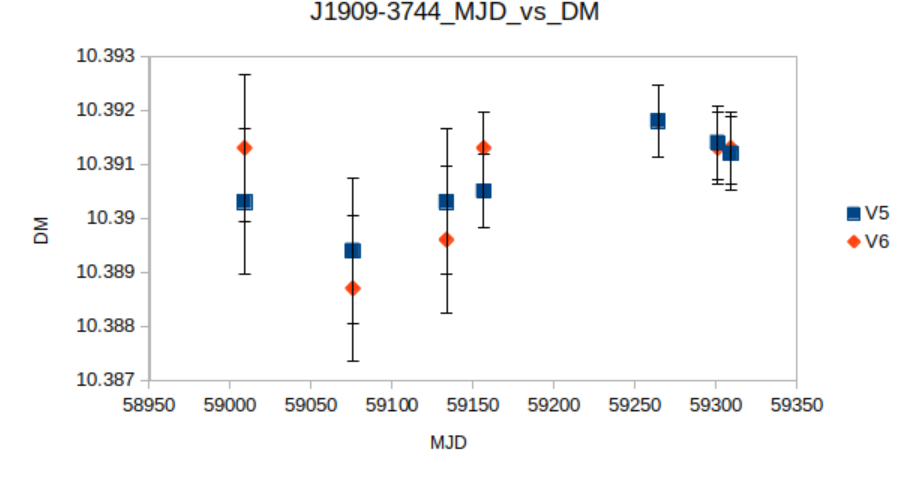
\includegraphics[width=1.1\linewidth]{Images/V2_8.png}
  \captionof{figure}{Result of using the {\tt pdmp} Analysis on J1909 Pulsar, with configuration as Bar = 1, Round = 1}
\end{minipage}
\end{figure}

\clearpage
\newpage
The initial task was succeeded by a complete reduction and processing, including profile comparison of J1713+0747 and J1939+2134 Pulsars. These test were much more explicit, in that they tested the complete processing to rule out any discrepancies outside of the Pinta processing. \\
\begin{figure}[htbp]
\begin{center}
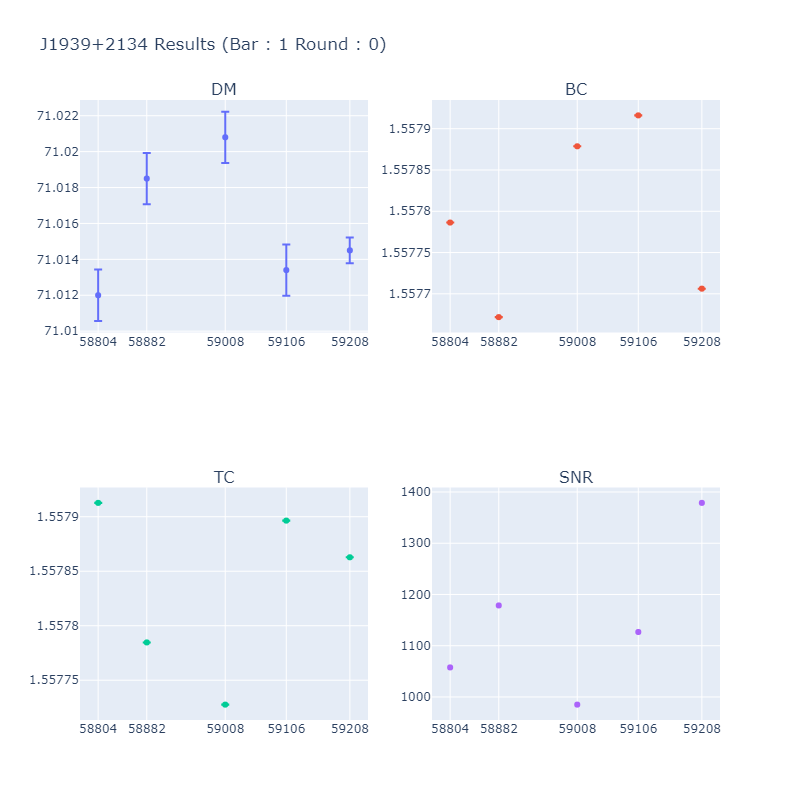
\includegraphics[height=12cm,width=14cm]{Images/Pulsar14.png}\\
\end{center}
\end{figure}
\\ DM Stands for Dispersion Measure, BC denotes Barycentric period, TC denotes Topocentric period and SNR denotes Signal to Noise Ratio. The processing results in a data sample output that looks as follows : (Note that this output is for a different pulsar epoch, mentioned as an example)

\begin{displayquote}
{\small \textsl{Best S/N = 204.66\\
BC MJD = 59106.664774\\
BC Period (ms) = 4.570535503  TC Period (ms) =  4.570474288  DM =   15.9910\\
Best BC Period (ms) = 4.570535454  Correction (ms) = -4.94526339e-08  Error (ms) = 7.424341696e-08\\
Best TC Period (ms) = 4.570474239  Correction (ms) = -4.945197141e-08  Error (ms) = 7.424341696e-08\\
Best DM =   15.9876  Correction = -0.00341  Error = 0.002095\\
Best BC Frequency (Hz) = 218.7927454  Error (Hz) = 3.554052078e-06\\
Pulse width (bins) = 13\\
Best Pdot =   0 s/s\\
Best Accn =   0 m/s\\}}
\end{displayquote}

\clearpage
\newpage
\subsection{DETERMINATION OF FREQUENCY SHIFT}
 This was taken up, upon coming across a realization that the DM of all Pulsars showed a jump near January 2021 at the same time, which pointed to an offset in either the processing or the observation semantics. A +10 KHz offset in the local oscillator settings was determined using this methodology. The following steps were followed to check for disparity in frequencies in the process.
\begin{enumerate}
    \item Find mean DM of J1713 pulsar before the jump event in Band 3.
    \item Substitute in the formula for LSB the parameters $F_{lo}$ as 0.5 (GHz),
$\Delta F$ as 0.2 (GHz), $N_{chan}$ = 256 and calculate $F_{1X}$ which is actually $\nu_{hi}$. (\cite{Susobhanan+2021})
\begin{center}
        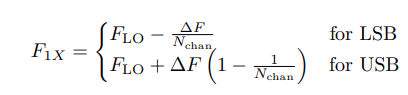
\includegraphics[height=2cm,width=8cm]{Images/Eqn.png}
\end{center}
    \item Use the formula $\nu_{lo} = \nu_{hi} - \Delta F$ to obtain $\nu_{lo}$
    \item Substitute in equation below, the values of DM1, $\nu_{lo}$ and
$\nu_{hi}$ as calculated above and calculate $\Delta t$ (\cite{10.12942/lrr-2008-8})
\end{enumerate}
\begin{center}
    $\Delta t = 4.15\;{\rm{ms}} \times \left[ {{{\left({{{{\nu _{{\rm{lo}}}}} \over {{\rm{GHz}}}}} \right)}^{- 2}} - {{\left({{{{\nu _{{\rm{hi}}}}} \over {{\rm{GHz}}}}} \right)}^{- 2}}} \right] \times \left({{{{\rm{DM}}} \over {{\rm{c}}{{\rm{m}}^{{\rm{- 3}}}}{\rm{pc}}}}} \right)$
\end{center}
Now, to find if there is a change in frequency, we will reverse this process with the DMs after the jump and obtain the 
\begin{enumerate}
    \item Now find mean DM2 of J1713 pulsar after the DM jump.
    \item Substitute $\Delta$ t calculated in the previous process, this DM2 and calculate
the factor in square bracket equation mentioned above. 
    \item Obtain the $\nu_{lo}$ and $\nu_{hi}$ values. This was done using the {\tt sympy} python library in python to solve the equation. The change in frequency is the difference in the values of $F_{LO}$.
    \item Repeat the same for J1909 pulsar, the results should be same for two pulsars in case of no frequency change.
\end{enumerate}

\subsection{RESULTS}
\begin{table}[htbp]
 \caption{Results obtained from calculation of frequency shift process}
  \centering
  \begin{tabular}{llllll}
    \toprule
    \cmidrule(r){1-4}
        & Pre-jump DM    &   $\Delta t$(ms) & Post-jump DM & $F_{LO}$(GHz)& $\Delta F$(GHz)\\
    \midrule\\ J1713 (V5)    & 15.998783   &  475.16733824824945  & \  15.997628 & 0.499991180113022 & 8.819886977984304e-06 \\\\
  \hline\\ J1713 (V6)   & 15.988197  & 474.8529317435362  &  15.986748 & 0.499988927659255 & 11.07234074498864e-06 \\\\
  \hline\\ J1909 (V5)   & 10.391595  & 308.6326338887038  &  10.391000 & 0.499993004791562 & 6.995208437998723e-06 \\\\
  \hline\\ J1909 (V6)   & 10.391048  & 308.6163878696146  &  10.390474 & 0.499993251330391 & 6.74866960898024e-06 \\\\
 \cmidrule(r){1-6}
  \end{tabular}
  \label{tab:table}
\end{table}
\newpage
\subsection{CONCLUSIONS}
The main conclusion was that \textbf{}{V6 Analysis was valid and can be used for science.}\\
It was seen that pdmp DMs and pat frequency match for all 4 cases. This suggested that .psrchive.cfg settings do not matter for DSPSR, but these matter in post-processing by psrchive (\cite{Hotan+2004}). For correct post-processing by psrchive, Bar 1 Round 0 config file is recommended.\\ \\
The GMRT Operations team issued a technical note which summarised the situation and its resolution as follows :\\
The DM jump appears to be due to a frequency shift in LO of +10 KHz in Cycle 39, Cycle 40.
For beam mode observations, The LO offset of 10 KHz introduces a systematic shift in frequencies interpreted by the analysis software. This can lead to an error in the DM estimates between 0.0005 to 0.001 pc$cm^-3$ and a residual DM smear in the time-series due to dedispersion to incorrect frequencies. This can also introduce a small shift in the time-of-arrival of data. The magnitude of these errors depend on DM of the source being observed and will vary from one source to another. It also depends on observing frequency. The most significant effect is likely in Band 3 and 4, while Band 5 data is not affected except for very large DM sources. The header for all data taken with TGC system prior to 29 July 2021 needs to be corrected by adding +10 KHz to the frequency in the header before carrying out the data reduction.\\
\newpage

\section{ACKNOWLEDGMENTS}
I am extremely grateful to Prof. Shantanu Desai for guiding me throughout this entire processes.  I am Grateful to Prof B.C. Joshi for allowing me to contribute to the InPTA team and for giving me guidance on very key aspects of my work. I would also like to thank to Jaikhomba Singha and Raghav Girgaonkar for showing me the ropes to the Process of Pulsar Analysis. 
Also, I am grateful to the observations team handling the uGMRT, who allowed me to obtain the necessary data for this work and to the entire InPTA consortium, which introduced me to this curious field of Pulsar Astronomy, and who made me feel included in this bold journey.
\newpage

% \bibliographystyle{unsrt}  
\printbibliography[title={\Large REFERENCES}]
\end{document}
